\pstart Pour faire comprendre parfaitement
[138 r\textsuperscript{o}] cette Hypothese, supposons dans
% \begin{wrapfigure}{l}{0.23\textwidth}                    
          %      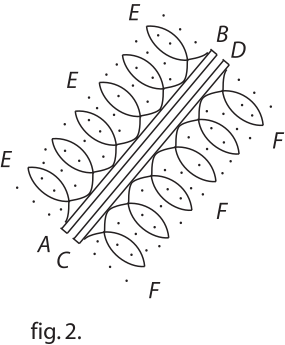
\includegraphics[width=0.23\textwidth]{images/37_3_138r2}\\\textit{[Fig. 1]}
                        %\caption{Bildbeschreibung}
             %           \end{wrapfigure}
                        %@ @ @ Dies ist eine Abstandszeile - fuer den Fall, dass mehrere figures hintereinander kommen, ohne dass dazwischen laengerer Text steht. Dies kann zu einer Fahlermeldung fuehren. @ @ @ \\
                     la \textso{fig. 2} deux \edtext{corps polis, dont les superficies interieures \textit{AB} et \textit{CD}}{\lemma{deux}\Afootnote{ \textit{ (1) }\ corps polis\protect\index{Sachverzeichnis}{corps!polis|textit} \textit{AB} et \textit{C} \textit{ (2) }\ corps [...] \textit{CD} \textit{ L}}}\footnote{\textit{In der rechten Spalte}: fig. 2 \textit{als Platzhalter für die fehlende Zeichnung.}} sont exactement contig\"{u}es, \edtext{lesquels soyent}{\lemma{}\Afootnote{lesquels soyent \textit{ erg.} \textit{ L}}} suspendus dans une liqueur ou matiere fluide \textit{EF}, toute troubl\'{e}e par une infinit\'{e} de vagues en tous sens et lignes\edtext{}{\lemma{}\Afootnote{lignes  \textbar\ sensibles \textit{ erg. u.}\  \textit{ gestr.}\ \textbar\ imaginables. \textit{ L}}} imaginables. Il est manifeste, que tous les coups que ces deux corps re\c{c}oivent des vagues de la liqueur contribuent \`{a} la conservation de leur contiguit\'{e} contre une separation directe; puisque tous les coups donnent contre les superficies \edtext{exterieures}{\lemma{superficies}\Afootnote{ \textit{ (1) }\ interieures \textit{ (2) }\ exterieures \textit{ L}}}, oppos\'{e}es l'une \`{a} l'autre, et font les corps estre pressez l'un vers l'autre. Car tous les coups que le corps \textit{AB} peut recevoir viennent d'\textit{E} vers \textit{F} et tous ceux qui rencontrent le corps \textit{CD} viennent de \textit{F} vers \textit{E}. Voila la substance de cette Hypothese. \edtext{\textso{L'Objection a est\'{e} faite, que cela seroit veritable}}{\lemma{\textso{L'Objection} [...] \textso{veritable:}}\Afootnote{\textit{am Rand doppelt angestrichen}}} si les corps \textit{AB}, et \textit{CD} estoient sans pores; mais comme ceux mêmes, qui introduisent cette matiere fluide\edtext{}{\lemma{}\Afootnote{fluide  \textbar\ invisible \textit{ gestr.}\ \textbar\ , plus \textit{ L}}}, plus subtile que l'air, luy font passage par les corps\protect\index{Sachverzeichnis}{corps!solide} les plus solides, il s'ensuit que les superficies interieures des corps contigûs, mais poreux, seront aussi frapp\'{e}es par le mouuement de la matiere.
                     \pend 
%Zeitz auskommentiert                     \begin{center}
%                     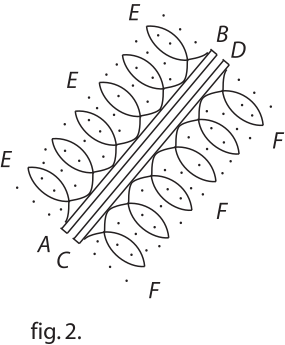
\includegraphics[width=0.35\textwidth]{images/37_3_138r2}
%                     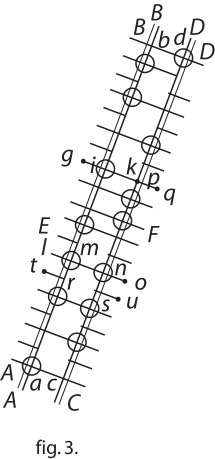
\includegraphics[width=0.3\textwidth]{images/37_3_138r3}\\\textit{[Fig. 1]}\hspace{4cm}\textit{[Fig. 2]}%\rule[0cm]{3cm}{0cm}
%                     \end{center}
                     \pstart  Car comme il \edtext{est \`{a} voir}{\lemma{il}\Afootnote{ \textit{ (1) }\ paroist \textit{ (2) }\ est \`{a} voir \textit{ L}}} dans\footnote{\textit{In der rechten Spalte}: fig. 3 \textit{als Platzhalter für die fehlende Zeichnung.}} la \textso{3}\textsuperscript{\textso{me}}\textso{ figure,}  toutes les lignes
                  %    \begin{wrapfigure}{l}{0.2\textwidth}                    
            %    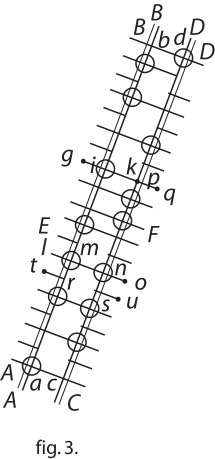
\includegraphics[width=0.2\textwidth]{images/37_3_138r3}\\\textit{[Fig. 2]}
                        %\caption{Bildbeschreibung}
             %           \end{wrapfigure}
                        %@ @ @ Dies ist eine Abstandszeile - fuer den Fall, dass mehrere figures hintereinander kommen, ohne dass dazwischen laengerer Text steht. Dies kann zu einer Fahlermeldung fuehren. @ @ @ \\
                     \edtext{des vagues ou}{\lemma{}\Afootnote{ des vagues ou  \textit{ erg.} \textit{ L}}} du mouuement qui viennent du cost\'{e} d'\textit{E} comme \textit{gik} et \textit{lmno} et qui passent par les pores du corps \textit{AB} comme \textit{i} vel \textit{m} rencontrent necessairement \textso{ou} un autre pore \edtext{\textso{ou} la superficie interieure du dit corps \textit{CD} a un endroit solide et sans pore comme \textit{k}}{\lemma{pore}\Afootnote{ \textit{ (1) }\ dans le corps oppos\'{e} \textit{CD} le coup de la vague \textit{lm} rencontre \textit{n} en quel cas  \textit{(a)}\ le coup de la vague \textit{(b)}\ ce coup passe outre   \textbar\ vers \textit{o} \textit{ erg.}\ \textbar\  sans s'arrêter ou contribuer \`{a} l'union ou desunion: \textso{ou} les lignes des coups \textit{ (2) }\ comme \textit{n} dans le corps oppos\'{e} \textit{CD}  \textit{(a)}\ comme \textit{(b)}\ ou la superficie interieure du dit corps oppos\'{e}, \textit{(c)}\ ou il est solide et sans pore. \textit{ (3) }\ \textso{ou} [...] \textit{CD} \textit{(a)}\ ou \textit{(b)}\ a [...] pore  \textbar\ comme \textit{k} \textit{ erg.}\ \textbar\  \textit{ L}}}. En premier cas si \edtext{la ligne du coup qui vient}{\lemma{si}\Afootnote{ \textit{ (1) }\ les coups \textit{ (2) }\ les lignes des coups qui viennent \textit{ (3) }\ la [...] vient \textit{ L}}} du cost\'{e} d'\textit{E} \edtext{comme \textit{lmno}, et qui passe par un pore}{\lemma{comme}\Afootnote{ \textit{ (1) }\ \textit{gik} et \textit{lmno}, et qui passent par les pores \textit{ (2) }\ \textit{lmno}, [...] pore \textit{ L}}} du corps \textit{AB} comme par \edtext{\textit{m} rencontre aussi un pore comme \textit{n} dans le corps oppos\'{e} \textit{CD}}{\lemma{par}\Afootnote{ \textit{ (1) }\ \textit{i} vel \textit{m} rencontrent dans le corps oppos\'{e} \textit{CD} \textit{ (2) }\ \textit{m} [...] \textit{CD} \textit{ L}}}; alors le choc du coup \textit{lmn} passe outre vers \textit{o} sans s'arrester aux corps, et sans contribuer \`{a} leur union ny desunion. Mais en dernier cas si la ligne du coup \edtext{qui vient du cost\'{e} d'\textit{E} et passe par le pore \textit{i} comme \textit{gi}, donne contre \textit{k}}{\lemma{coup}\Afootnote{ \textit{ (1) }\ \textit{gik} \textit{ (2) }\ qui vient du cost\'{e} d'\textit{E}   \textbar\ et [...] \textit{i} \textit{ erg.}\ \textbar\  comme \textit{gi}, donne contre \textit{k} \textit{ L}}} endroit solide et sans pore de la superficie interieure du corps oppos\'{e}e \textit{CD} ce coup, et tout autre de cette nature repoussant le corps \textit{CD} vers \textit{F} sans toucher au corps \textit{AB} tachera de separer le corps \textit{CD} du corps \textit{AB} et contribuera \`{a} leur desunion.
                     \pend
                      